\documentclass[cn,12pt]{elegantbook}

%插入图片包
\usepackage[graphicx]{realboxes}
\usepackage{subfigure}
\usepackage{float}


\usepackage{ulem}%插入删除线包

\title{从零开始}
\author{S.K.}
\date{October 1, 2023}
\cover{1.jpg}



\begin{document}

\maketitle
\frontmatter
\tableofcontents%命令输出论文目录
\mainmatter
\chapter{从零开始}
\begin{introduction}

    \item 三极管~\ref{jichen}
\end{introduction}
\section{集成} \label{jichen}
模电、数电的教材可以说大致介绍了最基本的逻辑和原理(教材是指《模拟电子技术基础》和《数字电子技术基础》)。
而电路分析相关的研究提供了坚实的理论依据。

\subsection{基础元件}
PN结(P11):具有单向导电性。

普通二极管(P15):包装PN结制成的电器元件。

稳压二极管(P20):用到了二极管的反向伏安特性。

光电二极管(P22):正常和二极管无异,光照后,等效附加电流源。

晶体三极管(P24):PNP型、NPN型,电流由P指向N。

共发射极放大电路(P25):使晶体管工作在放大状态的外部条件是发射结正向偏置且集电结反向偏置。

\begin{definition}[]

    共射交流电流放大系数  $\beta : \beta=\frac{\Delta i_C}{\Delta i_B}$

    $I_E =I_C +I_B $

    共基交流电流放大系数  $\alpha : \alpha=\frac{\Delta i_C}{\Delta i_E} =\frac{\beta }{1+\beta }$




\end{definition}

共集电极放大电路:

\begin{note}
整个模拟电路的教材,感觉是围绕放大电路展开,\sout{令人头大。}
打算从电路开始学习:
\end{note}


\subsection{电路分析}

基尔霍夫定律: $\sum \dot{u}=0$、$ \sum \dot{i} = 0$

节点电压法:技如其名

环路电流法:技如其名

叠加定理:一个电路,
可以看作每个独立电压源和电流源单独作用后叠加的结果。

替换定理:一个二端口电路,可以用电压源或电流源替代。

戴维南定理:等效电压法

诺顿定理:等效电流法








\chapter{小车的逻辑}

\section{准备}

车模、主控芯片(TC264)、传感器(不能自带MCU)、
母板(自行焊接,铺铜层印队伍名称)、
驱动板(可自行焊接,也可成品)、
电池(动力电池除外)、
电机不限(车模自带就可以)

    \begin{figure}[H]
        %\centering
        \subfigure{
        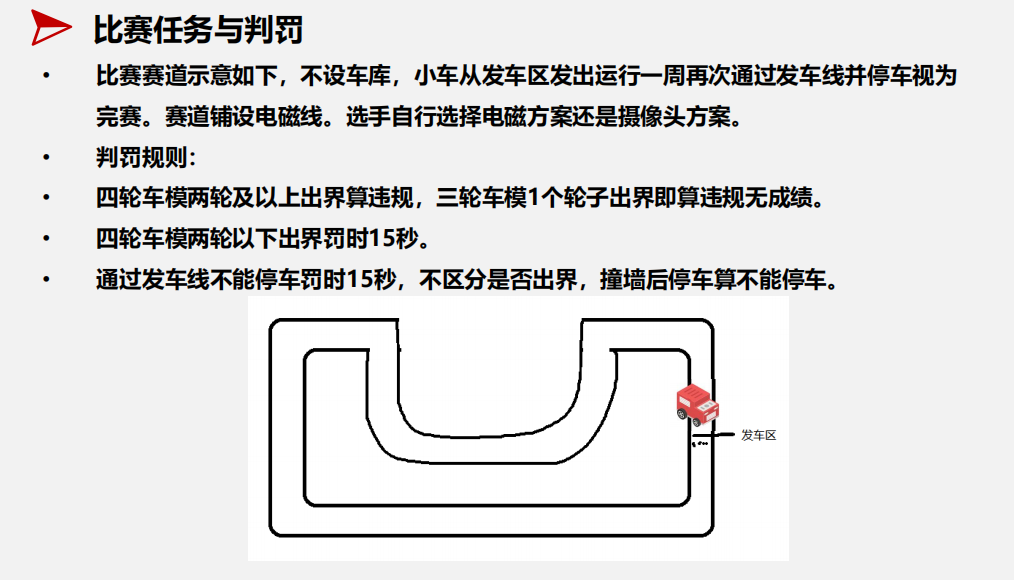
\includegraphics[width=0.4\textwidth,height=0.2\textheight]{规则.png} 
        }
        \hspace{4em}
        \subfigure{
        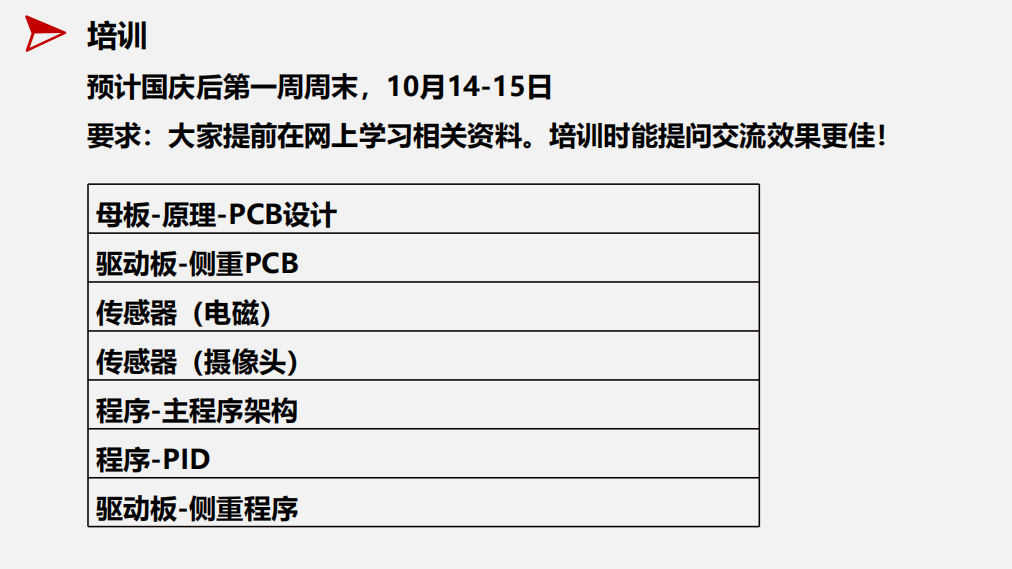
\includegraphics[width=0.4\textwidth,height=0.2\textheight]{./培训.png}
        }
        \caption{宣传截图}%这里是图片说明
    \end{figure}




\section{步骤}



\appendix

\chapter{自然资料}

\section{智能小车入门}
算法入门:

(一)姿态解算

	1.线性卡尔曼滤波

	2.互补滤波

	3.四元素姿态

	4.mpu6050的DMP的优劣

	5.如何获得稳定准确的yaw角

	6.基于硬件SPI使用ICM20602完成pitch,yaw,roll的高精度解算

(二)图像

	1.大津法

	2.固定阈值

	3.sobel算子

	4.阳光算法

(三)控制

	1.传统PID(增量式与位置式)

	2.LQR

电路设计入门:

(一)电源

	1.DCDC开关电源设计

	2.DCDC与LDO的异同与各自优点

	3.如何阅读芯片手册?

(二)立创EDA(标准版)使用方法与白嫖指南

(三)如何购买元器件?

(四)多层板设计与PCB LAYOUT

(五)驱动电路H桥设计

	1.BTN7971B,HIP4082,DRV8701各自优点与不足

	2.功率电路lay out 与隔离

单片机基础:

1.SPI与I2C各自的优点、缺点、使用方法(硬件SPI与硬件I2C)

2.正交编码器与增量式编码器的区别

3.DMA使用

4.(进阶)RT-thread的使用(可加分或者参与特殊组别)

5.蓝牙、OLED/TFT/IPS、BTN7971B、总钻风驱动与使用方法

6.TIM的几种模式:PWM生成,定时器,编码器,捕获器等等配置方式与使用

控制模型:

1.平衡小车(串级PID)

2.电机控制(速度环与位置环)


\section{信息来源}
    公众号:    卓晴公众号、逐飞科技公众号、龙邱公众号

    B站:       逐飞科技

    CSDN:      卓晴

    码云gitee: https://gitee.com/seekfree

    淘宝:      逐飞科技、龙邱科技

    \subsection{野生资源}
    
    卢佰奇:

    https://ittuann.github.io/Awesome-IntelligentCarRace


\section{科研}
    对于大创、测控电路、智能车


    对于设计、研究,需要了解一些新的东西,
    比如论坛、期刊、论文,
    
    网络编程论坛:
    https://www.oschina.net/
    
    程序语言设计:
    https://www.educoder.net/


    
\end{document}